
A continuación se analizan cada una de las redes de compensación en los modos correspondientes usando las simulaciones obtenidas para los modos correspondientes indicados en el cuadro~\tableref{table:compensation_networks}, usando los circuitos mostrados en la figura~\figref{fig:fig_complete_circuit_loop}, la figura~\figref{fig:fig_complete_circuit_rf} y la figura~\figref{fig:fig_complete_circuit_step}.\\

Los estados simulados para los casos de modo de regulación de tensión, son:

\begin{itemize}
\item $10 \si[per-mode=symbol]{\volt}$ de salida para $R_{L} = 10 \si[per-mode=symbol]{\ohm}$, $1 \si[per-mode=symbol]{\ampere}$ de carga.

\item $1 \si[per-mode=symbol]{\volt}$ de salida para $R_{L} = 1 \si[per-mode=symbol]{\ohm}$, $1 \si[per-mode=symbol]{\ampere}$ de carga.
\end{itemize}

y los estados simulados para los casos de modo de regulación de corriente, son:

\begin{itemize}
\item $2 \si[per-mode=symbol]{\ampere}$ de salida para $R_{L} = 0 \si[per-mode=symbol]{\ohm}$ (cortocircuito).

\item $200 \si[per-mode=symbol]{\milli\ampere}$ de salida para $R_{L} = 0 \si[per-mode=symbol]{\ohm}$ (cortocircuito).
\end{itemize}



Los modos elegidos responden a ser los casos extremos en modo tensión y modo corriente, de esa manera se espera tener cubierto el espectro de posibles estados de funcionamiento de la fuente de alimentación.\\

Los valores de los componentes de las redes de compensación se analizan para el valor de diseño y dos valores mas, uno por debajo y otro por arriba, tratando de ver porque el valor de diseño es el mas adecuado.\\

El análisis primero consiste en evaluar la simulación de ganancia de lazo en función de la frecuencia, realizando un barrido de frecuencia con el comando \textbf{SPICE} \textit{.ac} y en forma paramétrica con los valores a comparar de las redes de compensación de a uno por vez, para obtener en cada estado los márgenes de fase y de ganancia como se describió en la sección~\sectref{sect_margins_explanation}. En esto cabe aclarar que el análisis es aproximado dado que los márgenes en algunos casos pueden no ser sufientes para garantizar la estabilidad, siendo necesarios para un análisis completo, diagramas de \textbf{Nyquist} y de \textbf{Root Locus}, sin embargo para esto sería necesario un análisis teórico completo que permita obtener las transferencias completas cosa que no corresponde al simple análisis de validación por simulación.\\

Luego también se observa la respuesta en frecuencia del circuito, realizando también un barrido de frecuencia con el comando \textbf{SPICE} \textit{.ac} y en forma paramétrica con los valores a comparar de las redes de compensación de a uno por vez, de esta simulación se obtiene principalmente el ancho de banda del circuito.\\

Finalmente se observa la simulación de la respuesta del circuito a un salto de carga, según el modo analizado, esto equivale a una respuesta al escalón para este circuito, donde se puede ver si la respuesta es la esperada para un circuito estable, y evaluar si los sobre-picos presentes son aceptables.\\







\clearpage


%\\\\\\\\\\\\\\\\\\\\\\\\\\\
\subsection{Red de compensación Ccomp/Rcomp}

La red formada por \textbf{Ccomp} y \textbf{Rcomp} actúa tanto para el lazo de tensión como para el de corriente, por lo que se analizan ambos modos.

\clearpage



\subsubsection{Variación de la ganancia de lazo con Ccomp en modo tensión}



\begin{figure}[H] %htb
\begin{center}
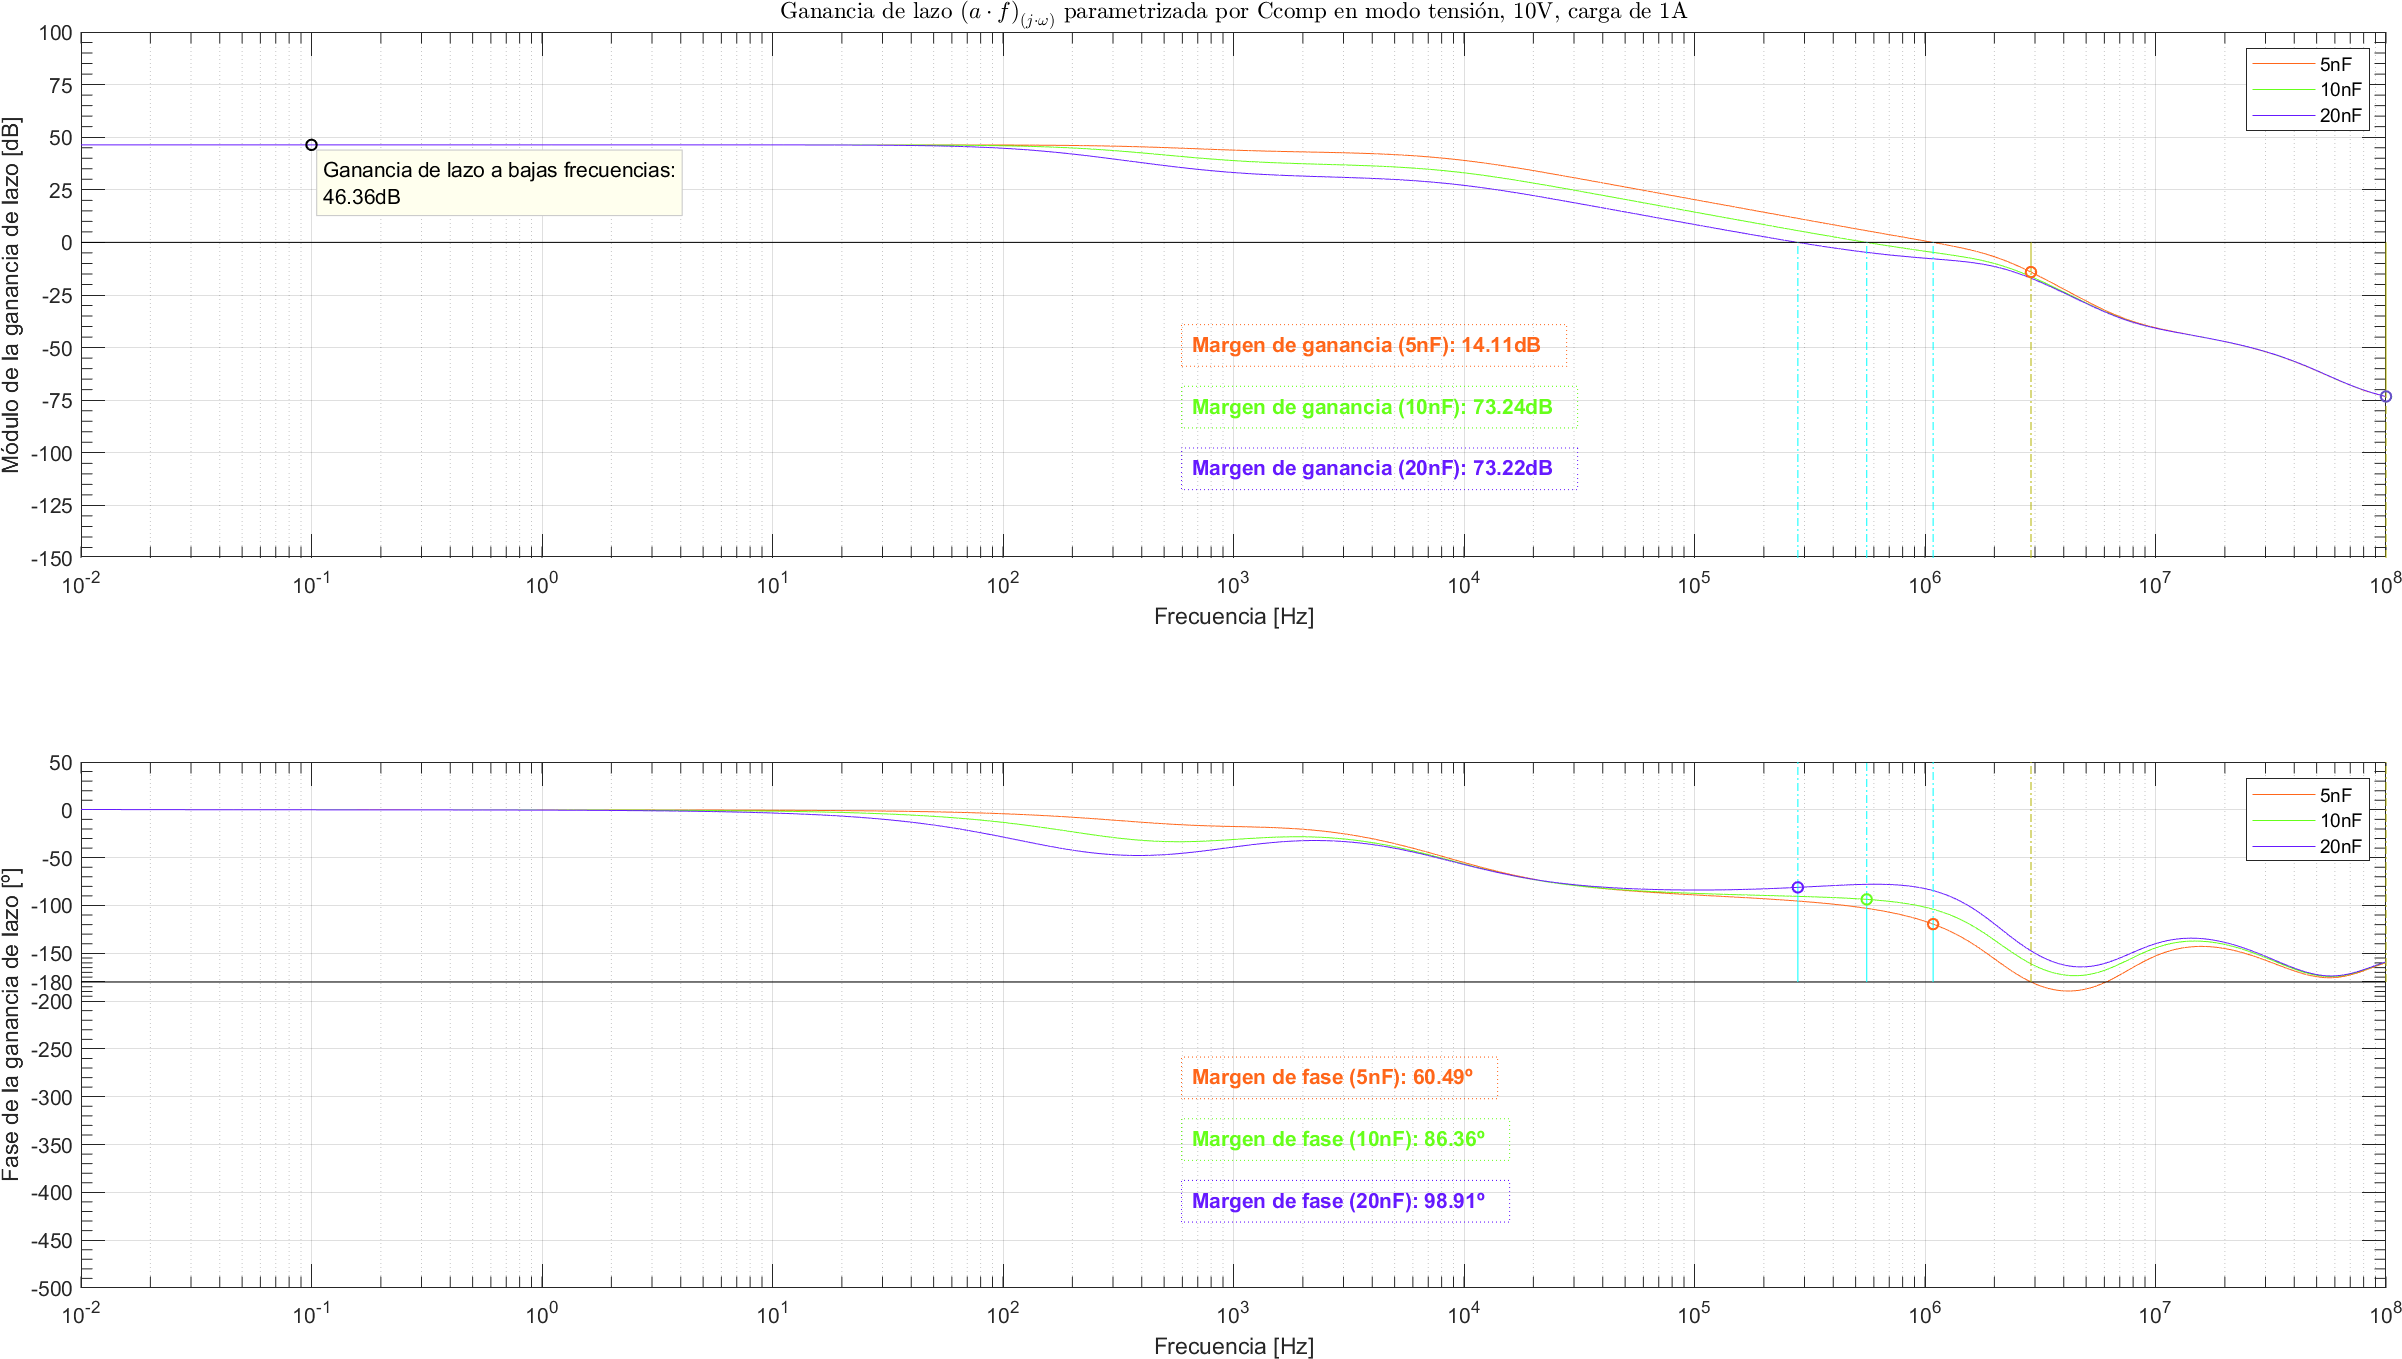
\includegraphics[width=1.1 \textwidth, angle=90]{./img/plots/loop/power_supply_CCOMP_LOOP_Modo1.png}
\caption{\label{fig:fig_power_supply_CCOMP_LOOP_Modo1}\footnotesize{Ganancia de lazo en función de la frecuencia parametrizada por Ccomp.}}
\end{center}
\end{figure}

\clearpage


\clearpage
%\\\\\\\\\\\\\\\\\\\\\\\\\\\




